\chapter{Concept}
This chapter presents the detailed conceptual design of the proposed architecture. It explains how the different components of the system interact with each other and how they come together to form a cohesive solution.

\section{The Collaboration Paradigm}

The Optimization Modeler provides a built-in multi-user collaboration architecture. Our approach builds upon this existing infrastructure in order to preserve modularity and ensure that legacy code remains untouched. In this section, we first describe how collaboration between human users is realized and then explain how the AI agent integrates into the same collaborative workflow.

\subsection{Human-to-Human Collaboration}

Collaboration between human users is initiated by a master user \cite{MarkoThesisMsc}, who registers and logs into the optimization platform hosted at \url{https://optimized.mpi-inf.mpg.de/modeler/}. After logging in, the master user creates a new modeling workspace and initiates a collaborative session.

To start collaboration, the user clicks the \emph{Share} button located at the bottom of the interface. This action opens a dialog containing shareable links for the current workspace. Two types of links are provided:
\begin{itemize}
    \item an \textbf{edit link}, which grants full editing privileges, and
    \item a \textbf{read link}, which grants view-only access.
\end{itemize}

Depending on the intended role of the invited participant, the master user shares either the edit link or the read link. This mechanism enables fine-grained access control while maintaining a lightweight collaboration setup.

\subsection{AI Agent Integration into the Collaborative Workspace}

The AI agent is deployed as a backend service and joins the collaborative workspace in a manner analogous to a human participant. The agent is provided with access to a web browser instance on the server through a web automation framework.

When the AI agent is invited to a workspace, a browser instance is automatically launched on the server. Authentication is performed using a dedicated account that represents the AI agent, after which the edit link is visited to open the shared modeling workspace. As this browser instance runs on the server, the Document Object Model (DOM) of the application can be accessed directly via JavaScript APIs. This enables the AI agent to observe, interact with, and modify the workspace in real time, using the same interface mechanisms available to human users.


\section{Schema Validation}
The output generated by the large language model (LLM) follows an XML-like syntax that is used internally by the Optimization Modeler. This syntax must conform to a predefined grammar that specifies the allowed constructs, constraints, and structural rules.

One of the major limitations of LLM-based systems is the possibility of hallucinations, meaning that the model may generate syntactically or structurally invalid output. Therefore, before any generated output is applied to the DOM, it must be validated.

To address this, we introduce a validation layer that checks the LLM-generated output against a formally defined grammar. An XML validator is used to verify whether the output conforms to the schema. In the case of validation errors, the error messages are fed back to the model, and the generation process is repeated until a syntactically valid and parsable output is produced. This mechanism prevents invalid or hallucinated outputs from being applied to the workspace.

\section{Human-in-the-Loop}
Once the LLM-generated output has been validated and applied to the DOM, the user is presented with multiple options. The user may accept the changes and make them permanent, reject the changes—thereby discarding them entirely and reverting to the previous model state—or provide additional feedback through the chat interface.

The AI agent uses this feedback, together with the current state of the optimization model, to iteratively refine its solution. The revised output is then validated and applied to the DOM again. This process continues until the user either accepts or rejects the final solution. This human-in-the-loop mechanism ensures continuous user oversight and provides fine-grained control over the modeling process.

\section{System Workflow}
The overall system workflow proceeds as follows. Once the AI agent joins the workspace, a chat interface becomes visible to the user, enabling direct communication with the agent. Through this interface, the user can request model modifications, seek assistance, or ask questions related to the optimization model.

Each user request is sent to the AI model along with the current state of the optimization model. The LLM interprets the natural language input and generates the corresponding output. Since the backend has access to the DOM of the modeler instance, the validated output can be applied directly to the workspace.

After the changes are applied, the user observes the updated model in their instance of the Optimization Modeler. The human-in-the-loop mechanism then allows the user to further refine, accept, or reject the generated changes before they are finalized.

\begin{figure}[t]
  \centering
  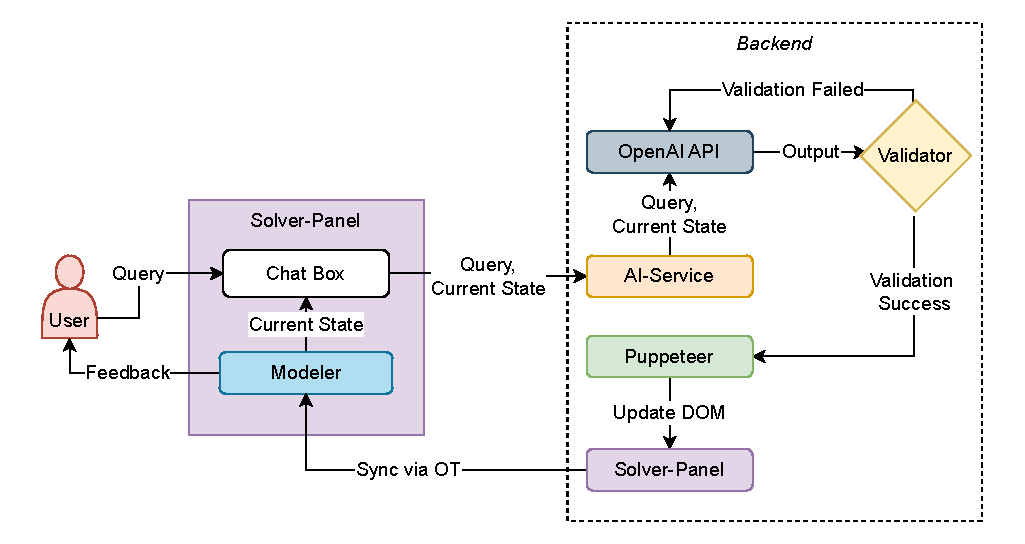
\includegraphics[width=10cm]{static/new.pdf}
  \caption{Overview of the proposed LLM architecture.}
  \label{fig:architecture}
\end{figure}

